\chapter{Projekt i implementacja aplikacji}

\section{Funkcje aplikacji - diagram przypadków użycia}

\begin{figure} [H]
	\centering
	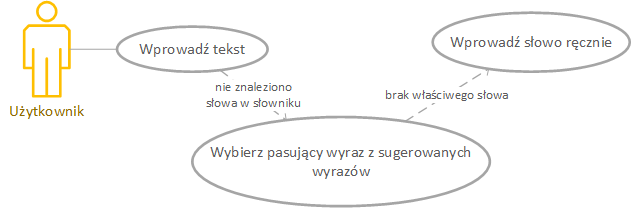
\includegraphics[width=1\linewidth]{rozdzial03/diagram.png}
	\caption{Diagram przypadków użycia}
	\label{fig:diagUzycia}
\end{figure}

Głównym zadaniem aplikacji jest wyszukiwanie błędnych wyrazów w języku polskim oraz ich korekcja. Aby tego dokonać aplikacja porównuje wyrazy znajdujące się w tekście z wyrazami znajdującymi się w słowniku. Jeśli danego słowa nie znaleziono zostaje ono uznane za błędne. Aby dokonać korekcji błędnych wyrazów stosowane są algorytmy opisane w poprzednich rozdziałach. Dla optymalizacji działania aplikacji wyszukiwanie sugestii odbywa się w osobnych wątkach co znacząco przyspiesza działanie aplikacji. 


\section{Interfejs aplikacji}

\begin{figure} [H]
	\centering
	\includegraphics[width=1\linewidth]{rozdzial03/screen1_1.png}
	\caption{Interfejs aplikacji}
	\label{fig:interfejs}
\end{figure}

\begin{enumerate}
	\item Ilość podpowiedzi - pozwala na ustawienie maksymalnej ilości podpowiedzi jakie mają się pojawić po kliknięciu prawym przyciskiem myszy na błędnie napisane słowo.
	\item Odległość Levenshteina - pozwala na ustawienie odległości jaka ma być brana pod uwagę w przypadku algorytmu Levenshteina. Im większa liczba tym więcej podpowiedzi ale jednocześnie zmniejsza to szybkość działania aplikacji ze względu na dodatkowe obliczenia które muszą zostać wykonane. 
	\item Ilość zmian - pozwala na ustawienie parametru ilości zmian dla algorytmu podmieniającego znaki diakrytyczne. Im większa liczba tym więcej podpowiedzi oraz dłuższy czas wykonywania algorytmu.
	\item Edytor tekstu - pozwala na edycję tekstu. Wyszukiwanie błędów działa w czasie rzeczywistym (funkcja sprawdzająca poprawność uruchamia się z każdym kliknięciem spacji). Jeśli dane słowo zostało uznane za błędne zostaje zaznaczone kolorem czerwonym. Aby je poprawić należy kliknąć na nie prawym przyciskiem myszki. Zostanie wyświetlone menu kontekstowe zawierające możliwe zamienniki. Aby podmienić słowo wystarczy kliknąć na zamiennik. Możliwe jest również poprawienie tekstu ręcznie wpisując w miejscu błędnego słowa poprawne. 
	
\end{enumerate}

\section{Wpływ parametrów na wyniki wyszukiwania}

\begin{figure} [H]
	\centering
	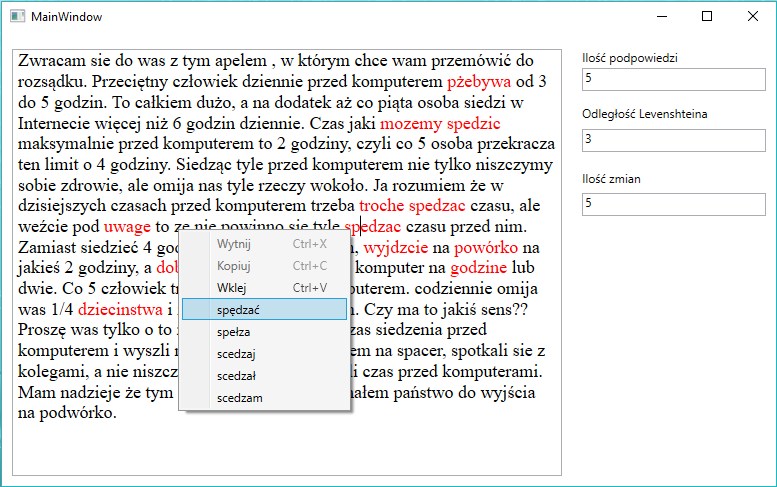
\includegraphics[width=1\linewidth]{rozdzial03/screen2.png}
	\caption{Przykładowy wynik wyszukiwania sugestii}
	\label{fig:interfejs1}
\end{figure}

\begin{figure} [H]
	\centering
	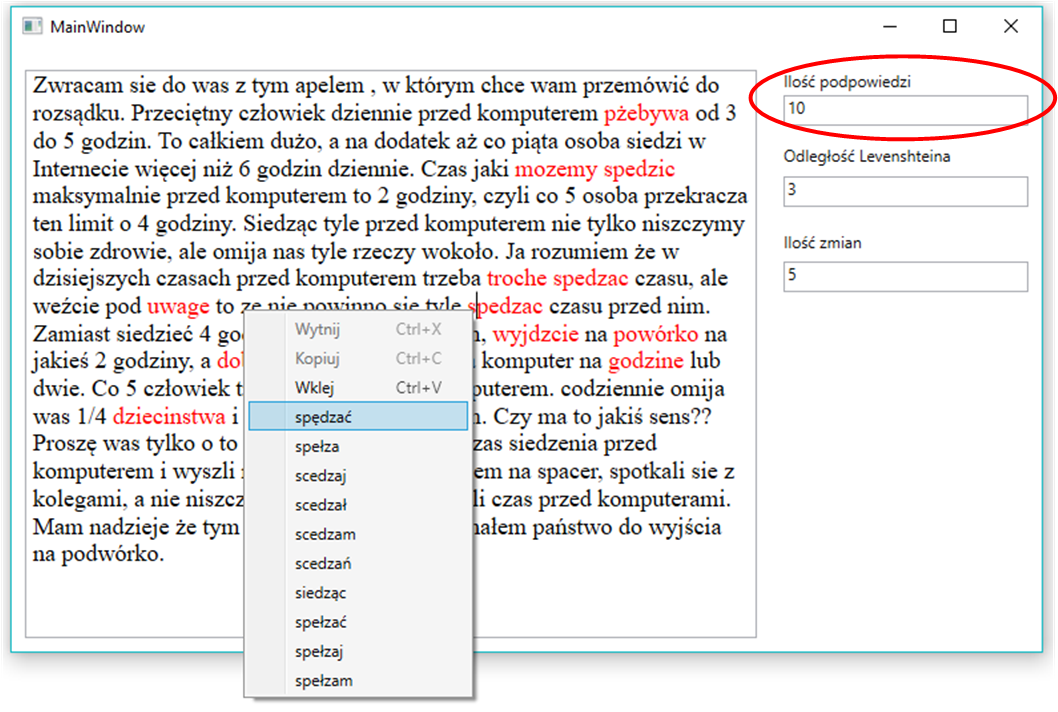
\includegraphics[width=1\linewidth]{rozdzial03/screen3_1.png}
	\caption{Zwiększenie ilości wyświetlanych sugestii}
	\label{fig:interfejs2}
\end{figure}

\begin{figure} [H]
	\centering
	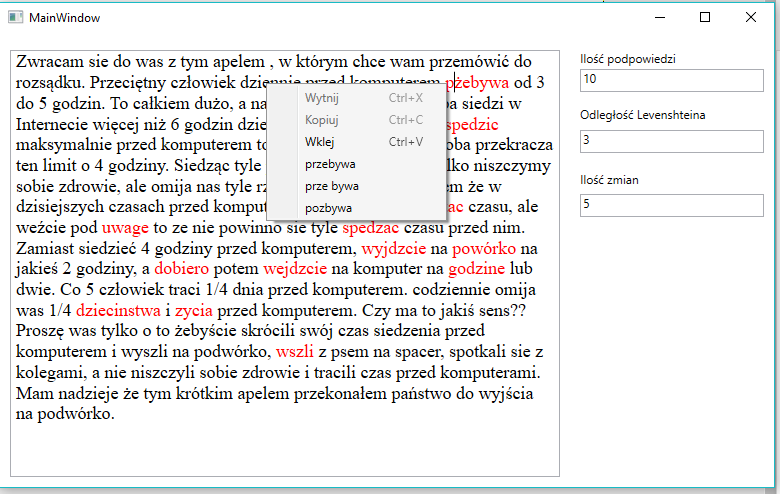
\includegraphics[width=1\linewidth]{rozdzial03/screen4.png}
	\caption{Przykładowy wynik wyszukiwania sugestii dla małej ilości podpowiedzi}
	\label{fig:interfejs3}
\end{figure}

\begin{figure} [H]
	\centering
	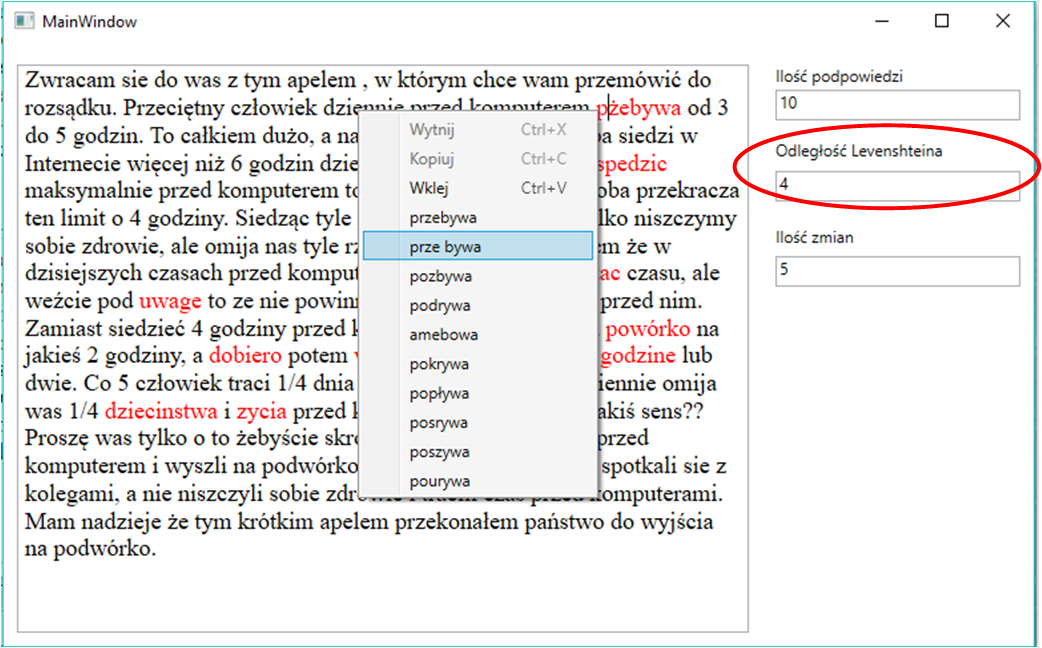
\includegraphics[width=1\linewidth]{rozdzial03/screen5_1.png}
	\caption{Zwiększenie odległości Levenhstaina}
	\label{fig:interfejs4}
\end{figure}

\begin{figure} [H]
	\centering
	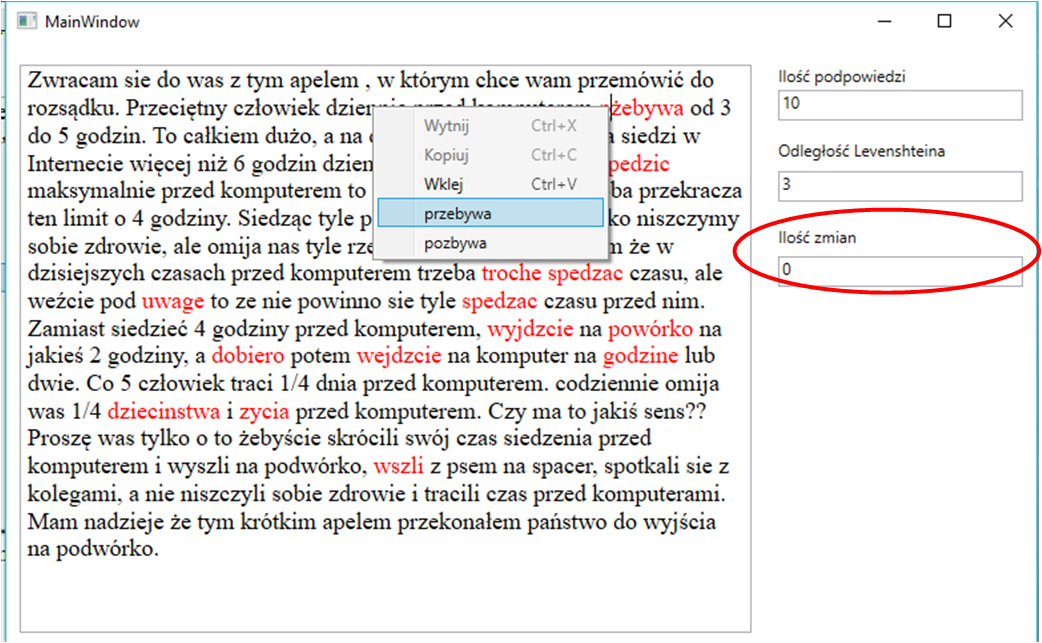
\includegraphics[width=1\linewidth]{rozdzial03/screen6_1.png}
	\caption{Zwiększenie ilości zmian}
	\label{fig:interfejs5}
\end{figure}

Odpowiednio zmieniając parametry znajdujące się w prawej części okna aplikacji można dostosować wyszukiwanie do potrzeb użytkownika. Rysunek \ref{fig:interfejs1} przedstawia przykładowe wyniki wyszukiwania podpowiedzi. Jeśli ilość wyświetlanych wyników nie jest odpowiednia można zmienić ich ilość tak aby uzyskać satysfakcjonujący wynik. Rysunek \ref{fig:interfejs2} przedstawia wpływ zwiększenia ilości wyświetlanych podpowiedzi. Jednocześnie ilość podpowiedzi nie ma wpływu na szybkość działania aplikacji. 

Pozostałe parametry wpływają na podobieństwo sugestii do wprowadzonego błędnie słowa. Na rysunku \ref{fig:interfejs3} został przedstawiony przykładowy wynik wyszukiwania który przy danych parametrach nie wypełnia całej listy podpowiedzi. Na rysunku \ref{fig:interfejs4} zwiększono odległość Levenshteina tak aby uzyskać więcej sugestii. Natomiast na rysunku \ref{fig:interfejs5} całkowicie zminimalizowano wpływ algorytmu podmieniającego znaki tak aby pozbyć się niechcianych podpowiedzi zawierających spacje.
 
\section{Realizacja wybranych funkcjonalności}

\begin{figure} [H]
	\centering
	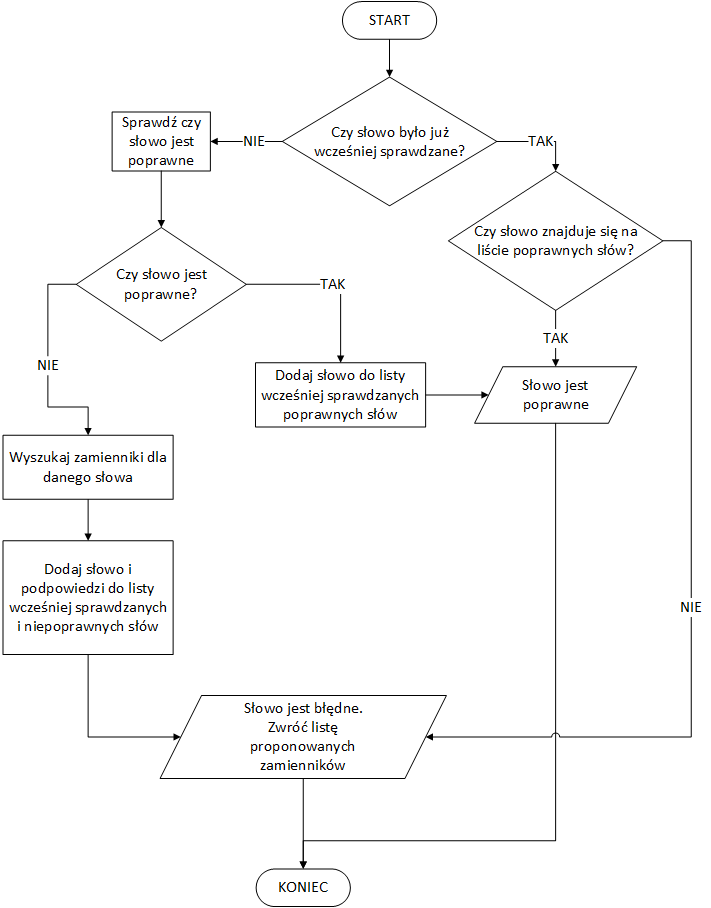
\includegraphics[width=1\linewidth]{rozdzial03/CorectorManager.png}
	\caption{Schemat korekcji tekstu z poziomu interfejsu}
	\label{fig:CorectorManager}
\end{figure}

\newpage

Główną funkcjonalnością aplikacji jest wyszukiwanie a następnie korekcja błędów. Rysunek~\ref{fig:CorectorManager} przedstawia schemat działania algorytmu odpowiedzialnego za powyższe zadanie. 

Początkowo algorytm sprawdza czy dane słowo było już wcześniej wyszukiwane. Jeśli tak to sprawdza czy jest ono na liście poprawnych słów. Jeśli tak to słowo jest poprawne i algorytm kończy pracę. Jeśli nie to sprawdza on listę błędnie wprowadzonych słów i zwraca on podpowiedzi. Jeśli podpowiedzi zostały już raz wyszukane dla danego słowa to zostają one zapisane. Ma to na celu przyspieszenie działania algorytmu ponieważ najwięcej czasu pochłania wyszukiwanie sugestii. 

Jeśli słowo jest wyszukiwane po raz pierwszy następuje sprawdzenie jego poprawności porównując je ze słowami znajdującymi się w słowniku. Jeśli jest poprawne to zostaje ono dodane do listy poprawnych sprawdzanych wcześniej słów i algorytm kończy pracę. Natomiast jeśli słowo jest błędne następuje wyszukiwanie sugestii. Po ich wyszukaniu zostają on zapisane wraz z niepoprawnym wyrazem na liście błędnych słów. Algorytm zwraca listę sugestii i kończy pracę.

Algorytm ten działa dla każdego słowa w osobnym wątku. Ma to za zadnie przyspieszenie działania aplikacji.  

\section{Optymalizacja}
\label{chap:optym}
Słownik użyty w projekcie składa się z blisko trzech milionów haseł. Podczas działania programu słownik ten musi być wielokrotnie przeglądany, zarówno poprzez sprawdzanie każdego wyrazu wpisanego przez użytkownika, jak i badaniu każdej powstałej kombinacji z algorytmu zamiany znaków jak i podziału na wyrazy oraz przy badaniu odległości Levenshteina w najprostszej wersji, każdy badany wyraz powinien mieć mierzoną odległość z każdym wyrazem znajdującym się w słowniku. Przy zwykłym użytkowaniu programu sprowadzałoby się to do wielu milionów operacji, a w związku z faktem iż założono w projekcie, że program ma działać możliwie w czasie rzeczywistym, podjęto próbę rozwiązania problemu z tak dużą liczbą operacji przeglądania całego słownika oraz z ograniczeniem ilości wykonywania obliczania odległości Levenshteina. W poniższych podrozdziałach opisane zostały podjęte w tym zakresie czynności.

\subsection{Serializacja}
Serializacja jest mechanizmem zamiany obiektu zapisywania obiektów, który pozwala na binarny zapis całego drzewa obiektów. Tak zapisany obiekt można w później uruchomić w dowolnym momencie pomijając cały etap tworzenia obiektów, a zastępując go procesem deserializacji, który z reguły powinien trwać szybciej niż proces tworzenia nowych obiektów. \\

W projekcie serializacja użyta została do zapisania klasy odpowiedzialnej za przechowywanie słownika. Przy pierwszym uruchomieniu programu słownik jest wczytywany z pliku tekstowego, a jego hasła są w odpowiedni sposób organizowane (więcej o tym w kolejnym podrozdziale). Dlatego uruchamianie programu i organizowanie słownika za każdym razem od nowa byłoby dość mało optymalne. Klasa z wczytanym słownikiem została zserializowana i zapisana do pliku. Od tego momentu przy każdym ponownym uruchomieniu programu, sprawdzane jest czy ten plik istnieje we wskazanym miejscu i o ile nikt go nie usunął to zostaje wczytany. Operacja trwa o wiele krócej, niż odczyt pliku i organizacja słownika na nowo. \\

Przy wyborze metody serializacji posłużono się artykułem ze strony [\ref{bib:serializ}], z którego to wynika, że jedną z najszybszych metod serializacji i deserializacji odbywa się z wykorzystaniem biblioteki \textit{ProtoBuf}, stworzonej przez firmę \textit{Google}. Metoda ta opera się o zapisywanie stanu klasy do pliku o strukturze XML, a każde pole i właściwość klasy musi zostać wyposażone w specjalny atrybut \textit{[ProtoMember(1)]} , przy czym cyfra podana w nawiasie musi być dla każdego pola unikalna ([\ref{bib:protbuf}]).

\subsection{Organizacja słownika}

Jak już zostało wspomniane w poprzednim podrozdziale, przy pierwszym uruchomieniu słownik jest wczytywany z pliku tekstowego i tworzona jest z niego klasa, która przechowuje słownik ten w odpowiednio zorganizowany sposób, który ułatwia jego przeszukiwanie. 

Hasła są w pamięci przechowywane w dwojaki sposób:
\begin{itemize}
	\item Jako zbiór list, z których każda przechowuje wyrazy o różnej długości oraz są posortowane w sposób alfabetyczny;
	\item Jako zbiór obiektów, z których każdy przechowuje wyrazy o różnej długości oraz rozpoczynające się na różną literę;
\end{itemize}

Pierwszy sposób przechowywania haseł został przystosowany specjalnie dla przeszukiwania słownika, poprzez przeglądanie haseł o wskazanej długości. Jest to szczególnie przydatne dla algorytmu wykorzystującego odległość Levenshteina. Badane słowo ma określoną długość, a zatem prawdopodobnie użytkownikowi również chodziło o słowo podobnej długości. Tak więc nie jest przeszukiwany cały słownik, a jedynie hasła o podobnej długości. W projekcie przyjęto że mogą to być hasła o długości z przedziału od -1 do +1 długości słowa badanego.

Drugi sposób przechowywania haseł został wykorzystany dla pozostałych dwóch algorytmów oraz dla sprawdzania czy dany wyraz znajduje się w słowniku. Przeszukiwanie słownika odbywa się w sposób dużo szybszy, gdyż znana jest długość słowa badanego oraz jego pierwsza litera, a oba te parametry odpowiadają indeksom dwuwymiarowego zbioru w którym przechowywane są hasła.

\subsection{Praca na wielu wątkach}

%TODO: PIRU

